\iffalse
\author{EE24BTECH11047}
\section{ee}
\chapter{2024}
\fi
\item If ‘$\rightarrow$’ denotes increasing order of intensity, then the meaning of the words
        [talk $\rightarrow$ shout $\rightarrow$ scream] is analogous to [please $\rightarrow$ \underline{\hspace{1cm}} $\rightarrow$ pander].
    Which one of the given options is appropriate to fill the blank?
    \begin{enumerate}
        \item flatter
        \item flutter
        \item fritter
        \item frizzle
    \end{enumerate}
\item P and Q have been allotted a hostel room with two beds, a study table, and an almirah. P is an avid bird-watcher and wants to sit at the table and watch birds outside the window. Q does not mind that as long as his bed is close to the ceiling fan.

Which one of the following arrangements suits them the most?
\begin{enumerate}
    \item \begin{figure}[!ht]
\centering
\resizebox{0.5\textwidth}{!}{%
\begin{circuitikz}
\tikzstyle{every node}=[font=\normalsize]
\draw  (3.75,10.75) rectangle (10.25,7.75);
\draw  (3.75,8.5) rectangle (5.5,7.75);
\draw  (3.75,10) rectangle (5.5,9.25);
\draw  (6,10.75) rectangle (7,10.25);
\draw  (9,10.75) rectangle (10.25,10.25);
\draw  (8.75,7.75) rectangle (10,7.5);
\draw  (5.25,10.75) rectangle (6.5,11);
\draw  (6.25,9.5) circle (0.5cm);
\node [font=\normalsize] at (5.75,11.25) {Window};
\node [font=\normalsize] at (6.5,10.5) {Table};
\node [font=\small] at (9.75,10.5) {Almirah};
\node [font=\normalsize] at (6.25,9.5) {Fan};
\node [font=\normalsize] at (4.5,9.5) {Bed Q};
\node [font=\normalsize] at (4.5,8) {Bed P};
\node [font=\normalsize] at (9.5,7.25) {Door};
\end{circuitikz}
}%

\label{fig:my_label}
\end{figure}
    \item \begin{figure}[!ht]
\centering
\resizebox{0.5\textwidth}{!}{%
\begin{circuitikz}
\tikzstyle{every node}=[font=\normalsize]
\draw  (3.75,10.75) rectangle (10.25,7.75);
\draw  (3.75,8.5) rectangle (5.5,7.75);
\draw  (8.5,10.75) rectangle (10.25,10);
\draw  (6,10.75) rectangle (7,10.25);
\draw  (8.75,7.75) rectangle (10,7.5);
\draw  (5.25,10.75) rectangle (6.5,11);
\draw  (6.25,9.5) circle (0.5cm);
\node [font=\normalsize] at (5.75,11.25) {Window};
\node [font=\normalsize] at (6.5,10.5) {Table};
\node [font=\small, rotate around={90:(0,0)}] at (4,10) {Almirah};
\node [font=\normalsize] at (6,9.5) {     Fan};
\node [font=\normalsize] at (9.25,10.25) {Bed Q};
\node [font=\normalsize] at (4.5,8) {Bed P};
\node [font=\normalsize] at (9.5,7.25) {Door};
\draw  (3.75,10.75) rectangle (4.25,9.5);
\end{circuitikz}
}%

\label{fig:my_label}
\end{figure}
\newpage
    \item \begin{figure}[!ht]
\centering
\resizebox{0.5\textwidth}{!}{%
\begin{circuitikz}
\tikzstyle{every node}=[font=\normalsize]
\draw  (3.75,10.75) rectangle (10.25,7.75);
\draw  (3.75,9.25) rectangle (5.25,8.5);
\draw [ rotate around={90:(9.875, 9.875)}] (9,10.25) rectangle (10.75,9.5);
\draw [ rotate around={90:(4, 10.25)}] (3.5,10.5) rectangle (4.5,10);
\draw  (8.75,7.75) rectangle (10,7.5);
\draw  (5.25,10.75) rectangle (6.5,11);
\draw  (6,9.25) circle (0.5cm);
\node [font=\normalsize] at (5.75,11.25) {Window};
\node [font=\normalsize, rotate around={90:(0,0)}] at (4,10.25) {Table};
\node [font=\small] at (8.25,10.5) {Almirah};
\node [font=\normalsize] at (5.75,9.25) {     Fan};
\node [font=\normalsize, rotate around={90:(0,0)}] at (10,10) {Bed Q};
\node [font=\normalsize] at (4.5,8.75) {Bed P};
\node [font=\normalsize] at (9.5,7.25) {Door};
\draw  (7.75,10.75) rectangle (9,10.25);
\end{circuitikz}
}%

\label{fig:my_label}
\end{figure}
    \item \begin{figure}[!ht]
\centering
\resizebox{0.5\textwidth}{!}{%
\begin{circuitikz}
\tikzstyle{every node}=[font=\normalsize]
\draw  (3.75,10.75) rectangle (10.25,7.75);
\draw [ rotate around={90:(10, 10.25)}] (9.5,10.5) rectangle (10.5,10);
\draw  (8.75,7.75) rectangle (10,7.5);
\draw  (5.25,10.75) rectangle (6.5,11);
\draw  (6,9.25) circle (0.5cm);
\node [font=\normalsize] at (5.75,11.25) {Window};
\node [font=\normalsize, rotate around={90:(0,0)}] at (10,10.25) {Table};
\node [font=\small] at (4.25,8) {Almirah};
\node [font=\normalsize] at (5.75,9.25) {     Fan};
\node [font=\normalsize] at (6.5,10.25) {Bed Q};
\node [font=\normalsize, rotate around={90:(0,0)}] at (4.25,9.75) {Bed P};
\node [font=\normalsize] at (9.5,7.25) {Door};
\draw  (3.75,8.25) rectangle (5,7.75);
\draw  (5.75,10.75) rectangle (7.25,10);
\draw  (3.75,10.75) rectangle (4.5,9.25);
\end{circuitikz}
}%

\label{fig:my_label}
\end{figure}
\end{enumerate}
\item The decimal number system uses the characters 0, 1, 2, \dots, 8, 9, and the octal number system uses the characters 0, 1, 2, \dots, 6, 7.

    For example, the decimal number 12 (= 1 $\times$ 10\textsuperscript{1} + 2 $\times$ 10\textsuperscript{0}) is expressed as 14 (= 1 $\times$ 8\textsuperscript{1} + 4 $\times$ 8\textsuperscript{0}) in the octal number system.

    The decimal number 108 in the octal number system is

    \begin{enumerate}
        \item 168
        \item 108
        \item 150
        \item 154
    \end{enumerate}

    \item A shopkeeper buys shirts from a producer and sells them at 20\% profit. A customer has to pay Rs.3,186.00 including 18\% taxes, per shirt. At what price did the shopkeeper buy each shirt from the producer?

    \begin{enumerate}
        \item Rs.2,500.00
        \item Rs.1,975.40
        \item Rs.2,700.00
        \item Rs.2,548.80
    \end{enumerate}

    \item If, for non-zero real variables \( x, y \), and real parameter \( \alpha > 1 \),
    \[
    x : y = (\alpha + 1) : (\alpha - 1),
    \]
    then, the ratio \( (x^2 - y^2) : (x^2 + y^2) \) is

    \begin{enumerate}
        \item \( 2\alpha : (\alpha^2 + 1) \)
        \item \( \alpha : (\alpha^2 + 1) \)
        \item \( 2\alpha : (\alpha^2 - 1) \)
        \item \( \alpha : (\alpha^2 - 1) \)
    \end{enumerate}
\item In the given text, the blanks are numbered (i)--(iv). Select the best match for all the blanks.

Following a row \underline{\hspace{1cm}} (i) the shopkeeper \underline{\hspace{1cm}} (ii) the price of a frying pan, the cook stood \underline{\hspace{1cm}} (iii) a row to withdraw cash \underline{\hspace{1cm}} (iv) the ATM booth.
\begin{enumerate}
    \item (i) with \hspace{1em} (ii) over \hspace{1em} (iii) at \hspace{1em} (iv) with
    \item (i) at \hspace{1em} (ii) over \hspace{1em} (iii) over \hspace{1em} (iv) in
    \item (i) with \hspace{1em} (ii) over \hspace{1em} (iii) in \hspace{1em} (iv) at
    \item (i) over \hspace{1em} (ii) with \hspace{1em} (iii) over \hspace{1em} (iv) at
\end{enumerate}

    \item In the following figure, 
    CD = 5 cm, BE = 10 cm, AE = 12 cm, 
    $\angle DAB = \angle DCB$, and $\angle DAE = \angle DBC = 90^\circ$.
    Points AFCD create a rhombus.
    \begin{figure}[!ht]
\centering
\resizebox{0.5\textwidth}{!}{%
\begin{circuitikz}
\tikzstyle{every node}=[font=\normalsize]
\draw  (6.25,10.5) -- (8,10.125) -- (9.75,10.5) -- (8,11) -- cycle;
\draw [short] (6.25,10.5) -- (9.75,10.5);
\draw [short] (8,11) -- (8,10);
\draw [short] (8,10) -- (8,7.75);
\draw [short] (6.25,10.5) -- (8,7.75);
\node [font=\normalsize] at (6,10.5) {A};
\node [font=\normalsize] at (7.75,10.3) {B};
\node [font=\normalsize] at (7.75,9.85) {F};
\node [font=\normalsize] at (8,11.25) {D};
\node [font=\normalsize] at (10,10.5) {C};
\node [font=\normalsize] at (8,7.5) {E};
\end{circuitikz}
}%

\label{fig:my_label}
\end{figure}
    The length of BF (in cm) is
    \begin{enumerate}
        \item  3
        \item  2
        \item  4
        \item  6
    \end{enumerate}
    \item The chart below shows the data of the number of cars bought by Millennials and Gen X people in a country from the year 2010 to 2020, as well as the yearly fuel consumption of the country (in Million liters).
     \begin{figure}[!ht]
    \centering
    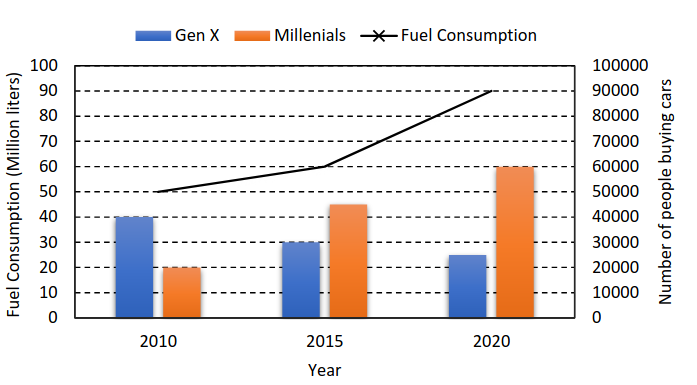
\includegraphics[width=5cm]{./GATE-yearwise/2024/figs/fig1.png}
    \end{figure}
    Considering the data presented in the chart, which one of the following options is true?
    
    \begin{enumerate}
        \item The percentage increase in fuel consumption from 2010 to 2015 is more than the percentage increase in fuel consumption from 2015 to 2020.
        \item The increase in the number of Millennial car buyers from 2015 to 2020 is less than the decrease in the number of Gen X car buyers from 2010 to 2015.
        \item The increase in the number of Millennial car buyers from 2010 to 2015 is more than the decrease in the number of Gen X car buyers from 2010 to 2015.
        \item The decrease in the number of Gen X car buyers from 2015 to 2020 is more than the increase in the number of Millennial car buyers from 2010 to 2015.
    \end{enumerate}
    \item The assembly shown has three teething circular objects (Pinions) and two teething flat objects (Racks), which are perfectly mating with each other. Pinions can only rotate clockwise or anti-clockwise, staying at their own center. Racks can translate towards the left ($\leftarrow$) or the right ($\rightarrow$) direction.

    If the object A (Rack) is translating towards the right ($\rightarrow$) direction, the correct statement among the following is:

\begin{figure}[!ht]
\centering
\resizebox{0.5\textwidth}{!}{%
\begin{circuitikz}
\tikzstyle{every node}=[font=\normalsize]
\draw [ fill={rgb,255:red,5; green,5; blue,5} ] (6.75,11.75) circle (1cm);
\draw [ fill={rgb,255:red,5; green,5; blue,5} , rotate around={-4:(6.875, 12.875)}] (6.75,13) rectangle (7,12.75);
\node [font=\normalsize] at (7.25,12.25) {};
\draw [ fill={rgb,255:red,5; green,5; blue,5} , rotate around={-32:(5.875, 12.375)}] (5.75,12.5) rectangle (6,12.25);
\draw [ fill={rgb,255:red,5; green,5; blue,5} , rotate around={-48:(7.625, 12.375)}] (7.5,12.5) rectangle (7.75,12.25);
\draw [ fill={rgb,255:red,5; green,5; blue,5} ] (7.75,11.75) rectangle (8,11.5);
\node [font=\normalsize] at (8.75,11) {};
\node [font=\normalsize] at (9.25,10.5) {};
\draw [ fill={rgb,255:red,5; green,5; blue,5} , rotate around={-142:(7.375, 10.875)}] (7.25,11) rectangle (7.5,10.75);
\node [font=\normalsize] at (9,10.5) {};
\draw [ fill={rgb,255:red,5; green,5; blue,5} , rotate around={-98:(6.625, 10.625)}] (6.5,10.75) rectangle (6.75,10.5);
\draw [ fill={rgb,255:red,5; green,5; blue,5} , rotate around={33:(5.875, 11.125)}] (5.75,11.25) rectangle (6,11);
\draw [ fill={rgb,255:red,5; green,5; blue,5} , rotate around={-173:(5.625, 11.625)}] (5.5,11.75) rectangle (5.75,11.5);
\draw [ fill={rgb,255:red,5; green,5; blue,5} ] (5.5,10.25) circle (0.75cm);
\node [font=\normalsize] at (7.25,10.25) {};
\node [font=\normalsize] at (7.25,10.25) {};
\draw [ fill={rgb,255:red,5; green,5; blue,5} , rotate around={2:(5.375, 11.125)}] (5.25,11.25) rectangle (5.5,11);
\draw [ fill={rgb,255:red,5; green,5; blue,5} , rotate around={52:(6.125, 10.875)}] (6,11) rectangle (6.25,10.75);
\node [font=\normalsize] at (6.5,10.25) {};
\node [font=\normalsize] at (6,10) {};
\draw [ fill={rgb,255:red,3; green,3; blue,3} , rotate around={-154:(4.75, 9.875)}] (5,10) rectangle (4.5,9.75);
\draw [ fill={rgb,255:red,3; green,3; blue,3} , rotate around={-23:(6.25, 9.875)}] (6.5,10) rectangle (6,9.75);
\draw [ fill={rgb,255:red,3; green,3; blue,3} , rotate around={90:(5.5, 9.375)}] (5.75,9.5) rectangle (5.25,9.25);
\draw [ fill={rgb,255:red,3; green,3; blue,3} , rotate around={-211:(4.75, 10.625)}] (5,10.75) rectangle (4.5,10.5);
\draw [ fill={rgb,255:red,10; green,10; blue,10} ] (6.75,9) circle (0.5cm);
\draw [ fill={rgb,255:red,3; green,3; blue,3} , rotate around={-54:(6.25, 9.375)}] (6.5,9.5) rectangle (6,9.25);
\node [font=\normalsize] at (6.75,9) {};
\draw [ fill={rgb,255:red,3; green,3; blue,3} , rotate around={-98:(6.75, 9.625)}] (7,9.75) rectangle (6.5,9.5);
\draw [ fill={rgb,255:red,3; green,3; blue,3} , rotate around={196:(7.25, 9.125)}] (7.5,9.25) rectangle (7,9);
\draw [ fill={rgb,255:red,3; green,3; blue,3} , rotate around={-23:(7.25, 8.625)}] (7.5,8.75) rectangle (7,8.5);
\draw [ fill={rgb,255:red,5; green,5; blue,5} , rotate around={-161:(6.375, 8.875)}] (6.75,9) rectangle (6,8.75);
\draw [ fill={rgb,255:red,3; green,3; blue,3} , rotate around={-85:(6.75, 8.375)}] (7,8.5) rectangle (6.5,8.25);
\draw [ fill={rgb,255:red,5; green,5; blue,5} ] (6,13.5) rectangle (9,13.25);
\draw [ fill={rgb,255:red,5; green,5; blue,5} ] (6.5,13.25) rectangle (6.25,12.75);
\draw [ fill={rgb,255:red,5; green,5; blue,5} ] (7.5,13.25) rectangle (7.25,12.75);
\draw [ fill={rgb,255:red,5; green,5; blue,5} ] (8,13.25) rectangle (7.75,12.75);
\node [font=\normalsize] at (8.5,12.5) {};
\draw [ fill={rgb,255:red,5; green,5; blue,5} ] (8.5,13.25) rectangle (8.25,12.75);
\draw [ fill={rgb,255:red,5; green,5; blue,5} ] (4.5,7.75) rectangle (7.5,7.5);
\draw [ fill={rgb,255:red,5; green,5; blue,5} ] (7.25,8.25) rectangle (7,7.75);
\draw [ fill={rgb,255:red,5; green,5; blue,5} ] (6.5,8.25) rectangle (6.25,7.75);
\draw [ fill={rgb,255:red,5; green,5; blue,5} ] (6,8.25) rectangle (5.75,7.75);
\draw [ fill={rgb,255:red,5; green,5; blue,5} ] (5.5,8.25) rectangle (5.25,7.75);
\draw [ fill={rgb,255:red,5; green,5; blue,5} ] (5,8.25) rectangle (4.75,7.75);
\node [font=\normalsize] at (7.25,13.75) {Object A $\rightarrow$};
\node [font=\normalsize] at (8.5,11.25) {Object P};
\node [font=\normalsize] at (3.75,10.25) {Object Q};
\node [font=\normalsize] at (8.25,9) {Object R};
\node [font=\normalsize] at (5.5,7) {Object B};
\end{circuitikz}
}%

\label{fig:my_label}
\end{figure}    
    \begin{enumerate}
        \item Object B translates towards the right direction.
        \item Object B translates towards the left direction.
        \item Object R rotates in the anticlockwise direction.
        \item Object Q rotates in the clockwise direction.
    \end{enumerate}
\item A surveyor has to measure the horizontal distance from her position to a distant reference point \( C \). Using her position as the center, a 200 m horizontal line segment is drawn with the two endpoints \( A \) and \( B \). Points \( A \), \( B \), and \( C \) are not collinear. Each of the angles \( \angle CAB \) and \( \angle CBA \) are measured as 87.8°. The distance (in m) of the reference point \( C \) from her position is nearest to

\begin{enumerate}
    \item 2603
    \item 2606
    \item 2306
    \item 2063
\end{enumerate}

\item Which one of the following matrices has an inverse?

\begin{enumerate}
    \item 
    \[
    \begin{pmatrix}
    1 & 4 & 8 \\
    0 & 4 & 2 \\
    0.5 & 2 & 4 
    \end{pmatrix}
    \]
    \item 
    \[
    \begin{pmatrix}
    1 & 2 & 3 \\
    2 & 4 & 6 \\
    3 & 2 & 9 
    \end{pmatrix}
    \]
    \item 
    \[
    \begin{pmatrix}
    1 & 4 & 8\\
    0 & 4 & 2\\
    1 & 2 & 4 
    \end{pmatrix}
    \]
    \item 
    \[
    \begin{pmatrix}
    1 & 4 & 8 \\
    0 & 4 & 2 \\
    3 & 12 & 24 
    \end{pmatrix}
    \]
\end{enumerate}
    \item The number of junctions in the circuit is
    \begin{figure}[!ht]
\centering
\resizebox{0.5\textwidth}{!}{%
\begin{circuitikz}
\tikzstyle{every node}=[font=\LARGE]
\draw (5.25,10.75) to[battery1] (5.25,8.75);
\draw (5.25,10.75) to[R] (7.25,10.75);
\draw (7.25,10.75) to[R] (9.25,10.75);
\draw (7.25,10.75) to[curved capacitor] (7.25,10.25);
\draw (7.25,10.25) to[R] (7.25,8.75);
\draw (5.25,8.75) to[curved capacitor] (7.25,8.75);
\draw (7.25,8.75) to[short] (9.25,8.75);
\draw (9.25,10.75) to[L ] (9.25,8.75);
\draw (10.75,10.75) to[curved capacitor] (10.75,6.75);
\draw (9.25,10.75) to[short] (10.75,10.75);
\draw (9.25,8.75) to[L ] (9.25,6.75);
\draw (9.25,6.75) to[short] (10.75,6.75);
\draw (7.25,6.75) to[R] (9.25,6.75);
\draw (7.25,8.75) to[R] (7.25,6.75);
\draw (5.25,8.75) to[L ] (5.25,6.75);
\draw (7.25,6.75) to[battery1] (5.25,6.75);
\end{circuitikz}
}%

\label{fig:my_label}
\end{figure}

    \begin{enumerate}
        \item 6
        \item 7
        \item 8
        \item 9
    \end{enumerate}
    \newpage    
    \item All the elements in the circuit are ideal. The power delivered by the 10 V source in watts is
\begin{figure}[!ht]
\centering
\resizebox{0.5\textwidth}{!}{%
\begin{circuitikz}
\tikzstyle{every node}=[font=\normalsize]
\draw (4,10.25) to[american voltage source] (4,7);
\draw (4,10.25) to[R] (6.75,10.25);
\draw (6.75,10.25) to[R] (6.75,7);
\draw (6.75,10.25) to[R] (9.5,10.25);
\draw (9.5,7) to[american current source] (9.5,10.25);
\draw (4,7) to[short] (9.5,7);
\node [font=\normalsize] at (5,10.75) {$\alpha$$\Omega$ };
\node [font=\normalsize] at (3.25,8.5) {10 V};
\node [font=\normalsize] at (6.25,8.5) {1$\Omega$ };
\node [font=\normalsize] at (8,10.75) {2$\Omega$ };
\node [font=\normalsize] at (10.25,8.5) {10 A};
\end{circuitikz}
}%

\label{fig:my_label}
\end{figure}
    \begin{enumerate}
        \item  0
        \item  50
        \item  100
        \item  dependent on the value of $\alpha$
    \end{enumerate}
